\documentclass{beamer}
\usetheme{Madrid}
\usepackage{lmodern}% http://ctan.org/pkg/lm
\setbeamersize{text margin left = 2.5em}
\setbeamersize{text margin right = 2.5em}
\usepackage{color}
\usepackage{graphicx}
\usepackage{MnSymbol}
\usepackage{amsmath}
\usepackage{comment}
\usepackage{tikz}
\usepackage{subfigure}
\usepackage{listings}
\usetikzlibrary{automata}

%\usepackage[backend=bibtex,sorting=none]{biblatex}
%\addbibresource{E:/Papers/LiuLab} %BibTeX�����ļ���λ��
%\setbeamerfont{footnote}{size=\tiny}
\setbeamertemplate{theorems}[numbered]
\setbeamertemplate{caption}[numbered]
%% ʹ�ý�ע���õ�Ƭijҳ���Ӳο����ס�
%% ��������ʹ�ã�\footfullcite{bib_item} %����item
%% \usepackage{anyfontsize}%% allowing font sizes at arbitrary sizes
\logo{
\includegraphics[height=0.05\textwidth]{Pic/logo}}
\newtheorem{df}{Definition}
\newtheorem{DF}{DEFINITION}
\newtheorem{prop}{Proposition}
\newtheorem{thm}{Theorem}
\newtheorem{cor}{COROLLARY}
\newtheorem{lm}{LEMMA}
% ----------------------------------------------------------------------------------------
% TITLE PAGE
% ----------------------------------------------------------------------------------------

\title{E05 SAT Problem}
% The short title appears at the bottom of every slide, the full title is only on the title page

\author{Suixin Ou} % Your name
\institute[SYSU] % Your institution as it will appear on the bottom of every slide, may be shorthand to save space
{
  School of Computer Science\\
  Sun Yat-sen University \\ % Your institution for the title page
  \medskip
  % Your email address
}

\date{October 26, 2021} % Date, can be changed to a custom date

\AtBeginSection[]
{
  \begin{frame}
    \tableofcontents[currentsection,currentsubsection]
  \end{frame}
}

\begin{document}

\begin{frame}
  \titlepage
\end{frame}

\begin{frame}
  \frametitle{Task}
  \begin{block}{Problem}
    \begin{itemize}
      \item In logic and computer science, the Boolean satisfiability problem (SAT) is the problem of determining if there exists an interpretation that satisfies a given Boolean formula.
      \item In other words, it asks whether the variables of a given Boolean formula can be consistently replaced by the values TRUE or FALSE in such a way that the formula evaluates to TRUE.
	  \item If this is the case, the formula is called satisfiable. On the other hand, if no such assignment exists, the function expressed by the formula is FALSE for all possible variable assignments and the formula is unsatisfiable. 
    \end{itemize}
      
    \begin{figure}[ht]
      \centering
      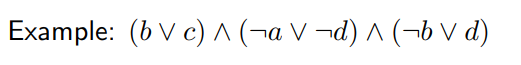
\includegraphics[width=0.3\textwidth]{Pic/example}
      \caption{SAT Problem}
    \end{figure}
  \end{block}
\end{frame}


\begin{frame}
  \frametitle{Task}
  \begin{block}{Input-output}
    \begin{itemize}
      \item Input: a cnf in "data.txt". 

	\begin{itemize}
	      \item The file "data.txt" starts with a line, "p cnf nbvar nbclauses", that indicates that the instance is in CNF format; nbvar is the exact number of variables appearing in the file; nbclauses is the exact number of clauses contained in the file.
	      \item Then the clauses follow. Each clause is a sequence of distinct non-null numbers between -nbvar and nbvar ending with 0 on the same line; it cannot contain the opposite literals i and -i simultaneously. 
		  \item Positive numbers denote the corresponding variables. Negative numbers denote the negations of the corresponding variables.
    \end{itemize}


      \item Output: an interpretation that satisfies the given CNF formula.
    \end{itemize}
  \end{block}
\end{frame}

\begin{frame}
  \frametitle{Task}
  \begin{block}{Submission}
    pack your report \texttt{E05\_YourNumber.pdf} and source code into zip file \texttt{E05\_YourNumber.zip}, then send it to \texttt{ai\_course2021@163.com}.
  \end{block}
\end{frame}

\begin{frame}
  \frametitle{Solution}
  Algorithm
  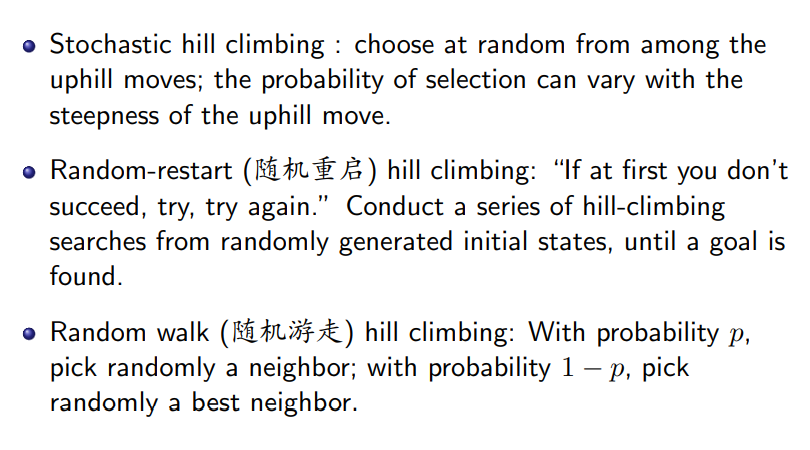
\includegraphics[width=1.0\textwidth]{Pic/algorithm}
\end{frame}




\begin{frame}
  \frametitle{Solution}
  \begin{columns}
    \begin{column}{.5\linewidth}
      Read input
      
      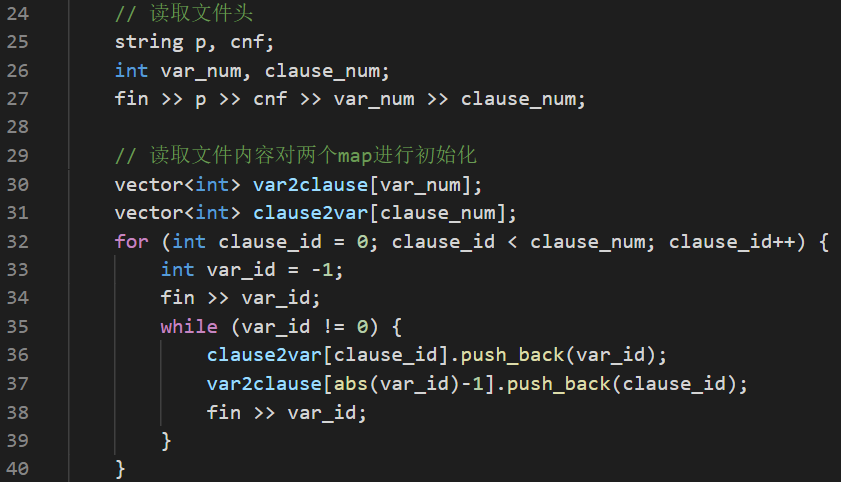
\includegraphics[width=1.0\textwidth]{Pic/read-input}

      Visualize output
      
      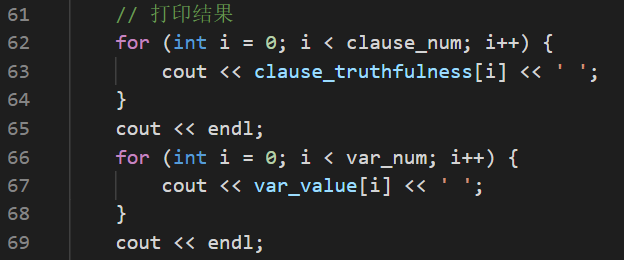
\includegraphics[width=1.0\textwidth]{Pic/visualize-output}
    \end{column}
    \begin{column}{.5\linewidth}
      check whether a clause is correct
      
      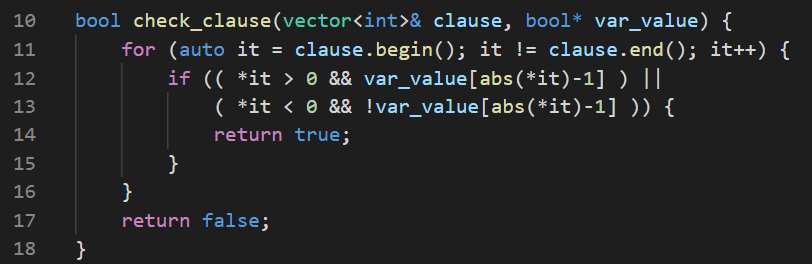
\includegraphics[width=1.0\textwidth]{Pic/check-clause}
    \end{column}
  \end{columns}

\end{frame}

\begin{frame}
  \frametitle{Solution}
      \textbf{You should finish the hill climbing algorithm with random start,}
      
      
\includegraphics[width=1.0\textwidth]{Pic/h1}

      \textbf{and random walk.}
      
      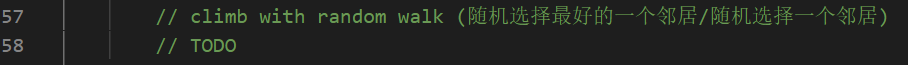
\includegraphics[width=1.0\textwidth]{Pic/h2}

\end{frame}
%-----------------------------------------------------------------------------------------

\begin{frame}
  \Huge{\centerline{The End}}
\end{frame}

% ----------------------------------------------------------------------------------------


\end{document}
